%%%%%%%%%%%%%%%%%%%%% chapter.tex %%%%%%%%%%%%%%%%%%%%%%%%%%%%%%%%%
%
% sample chapter
%
% Use this file as a template for your own input.
%
%%%%%%%%%%%%%%%%%%%%%%%% Springer-Verlag %%%%%%%%%%%%%%%%%%%%%%%%%%
%\motto{Use the template \emph{chapter.tex} to style the various elements of your chapter content.}

\chapter{Rosetta Code Tasks starting with E}

\section*{EBNF parser}

[aka \emph{Parse EBNF}]

Write a program that can parse a grammar in Extended Backus--Naur Form
and then parse something else according to the grammar. The program is
only required to decide whether or not the something else belongs to
the language described by the grammar, but for extra credit, it can
output a syntax tree. See \emph{the tests}.


\begin{wideverbatim}

(de EBNF
   "expr  : term ( ( PLUS | MINUS )  term )* ;"
   "term  : factor ( ( MULT | DIV ) factor )* ;"
   "factor   : NUMBER ;" )

(for E EBNF
   (use (@S @E)
      (unless (and (match '(@S : @E ;) (str E)) (not (cdr @S)))
         (quit "Invalid EBNF" E) )
      (put (car @S) 'ebnf @E) ) )


\end{wideverbatim}

\begin{wideverbatim}

(de matchEbnf (Pat)
   (cond
      ((asoq Pat '((PLUS . +) (MINUS . -) (MULT . *) (DIV . /)))
         (let Op (cdr @)
            (when (= Op (car *Lst))
               (pop '*Lst)
               Op ) ) )
      ((== 'NUMBER Pat)
         (cond
            ((num? (car *Lst))
               (pop '*Lst)
               @ )
            ((and (= "-" (car *Lst)) (num? (cadr *Lst)))
               (setq *Lst (cddr *Lst))
               (- @) ) ) )
      ((get Pat 'ebnf) (parseLst @))
      ((atom Pat))
      (T
         (loop
            (T (matchEbnf (pop 'Pat)) @)
            (NIL Pat)
            (NIL (== '| (pop 'Pat)))
            (NIL Pat) ) ) ) )


(de parseLst (Pat)
   (let (P (pop 'Pat)  X (matchEbnf P))
      (loop
         (NIL Pat)
         (if (n== '* (cadr Pat))
            (if (matchEbnf (pop 'Pat))
               (setq X (list @ X))
               (throw) )
            (loop
               (NIL *Lst)
               (NIL (matchEbnf (car Pat)))
               (setq X (list @ X (or (matchEbnf P) (throw)))) )
            (setq Pat (cddr Pat)) ) )
      X ) )

(de parseEbnf (Str)
   (let *Lst (str Str "")
      (catch NIL
         (parseLst (get 'expr 'ebnf)) ) ) )

Output:

: (parseEbnf "1 + 2 * -3 / 7 - 3 * 4")
-> (- (+ 1 (/ (* 2 -3) 7)) (* 3 4))


\end{wideverbatim}


\pagebreak{}
\section*{Echo server}

Create a network service that sits on TCP port \texttt{12321}, which
accepts connections on that port, and which echoes complete lines (using
a carriage-return/line-feed sequence as line separator) back to clients.
No error handling is required. For the purposes of testing, it is only
necessary to support connections from localhost (\texttt{127.0.0.1} or
perhaps \texttt{::1}). Logging of connection information to standard
output is recommended.

The implementation must be able to handle simultaneous connections from
multiple clients. A multi-threaded or multi-process solution may be
used. Each connection must be able to echo more than a single line.

The implementation must not stop responding to other clients if one
client sends a partial line or stops reading responses.



\begin{wideverbatim}

(setq Port (port 12321))

(loop
   (setq Sock (listen Port))           # Listen
   (NIL (fork) (close Port))           # Accepted
   (close Sock) )                      # Parent: Close socket and continue

# Child:
(prinl (stamp) " -- (Pid " *Pid ") Client connected from " *Adr)

(in Sock
   (until (eof)                        # Echo lines
      (out Sock (prinl (line))) ) )

(prinl (stamp) " -- (Pid " *Pid ") Client disconnected")
(bye)                                  # Terminate child

\end{wideverbatim}

\pagebreak{}
\section*{Element-wise operations}

Similar to \emph{Matrix multiplication} and \emph{Matrix
  transposition}, the task is to implement basic element-wise
matrix-matrix and scalar-matrix operations, which can be referred to
in other, higher-order tasks. Implement addition, subtraction,
multiplication, division and exponentiation.

Extend the task if necessary to include additional basic operations,
which should not require their own specialised task. 

\begin{wideverbatim}

(de elementWiseMatrix (Fun Mat1 Mat2)
   (mapcar '((L1 L2) (mapcar Fun L1 L2)) Mat1 Mat2) )

(de elementWiseScalar (Fun Mat Scalar)
   (elementWiseMatrix Fun Mat (circ (circ Scalar))) )

Test:

(let (S 10  M '((7 11 13) (17 19 23) (29 31 37)))
   (println (elementWiseScalar + M S))
   (println (elementWiseScalar - M S))
   (println (elementWiseScalar * M S))
   (println (elementWiseScalar / M S))
   (println (elementWiseScalar ** M S))
   (prinl)
   (println (elementWiseMatrix + M M))
   (println (elementWiseMatrix - M M))
   (println (elementWiseMatrix * M M))
   (println (elementWiseMatrix / M M))
   (println (elementWiseMatrix ** M M)) )

Output:

((17 21 23) (27 29 33) (39 41 47))
((-3 1 3) (7 9 13) (19 21 27))
((70 110 130) (170 190 230) (290 310 370))
((0 1 1) (1 1 2) (2 3 3))
((282475249 25937424601 137858491849) (2015993900449 6131066257801 ...

((14 22 26) (34 38 46) (58 62 74))
((0 0 0) (0 0 0) (0 0 0))
((49 121 169) (289 361 529) (841 961 1369))
((1 1 1) (1 1 1) (1 1 1))
((823543 285311670611 302875106592253) (827240261886336764177 ...

\end{wideverbatim}

\pagebreak{}
\section*{Empty program}

In this task, the goal is to create the simplest possible program that
is still considered ``correct.''

\begin{wideverbatim}

(de foo ())

\end{wideverbatim}

\pagebreak{}
\section*{Empty string}

Languages may have features for dealing specifically with empty strings
(those containing no characters).

The task is to:

\begin{itemize}
\item
  Demonstrate how to assign an empty string to a variable.
\end{itemize}

\begin{itemize}
\item
  Demonstrate how to check that a string is empty.
\item
  Demonstrate how to check that a string is not empty.
\end{itemize}


\begin{wideverbatim}

  The empty string is represented by
  '[http://software-lab.de/doc/ref.html#nilSym NIL]' in PicoLisp.
  During input, two subsequent double qoutes '""' return the symbol
  NIL.

# To assign a variable an empty string:
(off String)
(setq String "")
(setq String NIL)

# To check for an empty string:
(or String ..)
(ifn String ..)
(unless String ..)

# or a non-empty string:
(and String ..)
(if String ..)
(when String ..)

\end{wideverbatim}

\pagebreak{}
\section*{Ensure that a file exists}

In this task, the job is to verify that a file called ``input.txt'' and
the directory called ``docs'' exist. This should be done twice: once for
the current working directory and once for a file and a directory in the
filesystem root.


\begin{wideverbatim}

(if (info "file.txt")
   (prinl "Size: " (car @) " bytes, last modified " (stamp (cadr @) (cddr @)))
   (prinl "File doesn't exist") )

\end{wideverbatim}

\pagebreak{}
\section*{Enumerations}

Create an enumeration of constants with and without explicit values.

\begin{wideverbatim}

Enumerations are not very useful in a symbolic language like PicoLisp. If
desired, an 'enum' function could be defined:

(de enum "Args"
   (mapc def "Args" (range 1 (length "Args"))) )

: (enum A B C D E F)
-> F

: A
-> 1
: B
-> 2
: F
-> 6

\end{wideverbatim}

\pagebreak{}
\section*{Environment variables}

Show how to get one of your process's
\href{http://en.wikipedia.org/wiki/Environment\_variable}{environment
  variables}. The available variables vary by system; some of the
common ones available on Unix include PATH, HOME, USER.


\begin{wideverbatim}

: (sys "TERM")
-> "xterm"

: (sys "SHELL")
-> "/bin/bash"

\end{wideverbatim}

\pagebreak{}
\section*{Equilibrium index}


An equilibrium index of a sequence is an index into the sequence such
that the sum of elements at lower indices is equal to the sum of
elements at higher indices. For example, in a sequence \emph{A}:

\emph{A}\textsubscript{0} = − 7

\emph{A}\textsubscript{1} = 1

\emph{A}\textsubscript{2} = 5

\emph{A}\textsubscript{3} = 2

\emph{A}\textsubscript{4} = − 4

\emph{A}\textsubscript{5} = 3

\emph{A}\textsubscript{6} = 0

3 is an equilibrium index, because:

\emph{A}\textsubscript{0} + \emph{A}\textsubscript{1} +
\emph{A}\textsubscript{2} = \emph{A}\textsubscript{4} +
\emph{A}\textsubscript{5} + \emph{A}\textsubscript{6}

6 is also an equilibrium index, because:

\emph{A}\textsubscript{0} + \emph{A}\textsubscript{1} +
\emph{A}\textsubscript{2} + \emph{A}\textsubscript{3} +
\emph{A}\textsubscript{4} + \emph{A}\textsubscript{5} = 0

(sum of zero elements is zero)

7 is not an equilibrium index, because it is not a valid index of
sequence \emph{A}.

Write a function that, given a sequence, returns its equilibrium indices
(if any). Assume that the sequence may be very long.


\begin{wideverbatim}

(de equilibria (Lst)
   (make
      (let Sum 0
         (for ((I . L) Lst L (cdr L))
            (and (= Sum (sum prog (cdr L))) (link I))
            (inc 'Sum (car L)) ) ) ) )

Output:

: (equilibria (-7 1 5 2 -4 3 0))
-> (4 7)

: (equilibria (make (do 10000 (link (rand -10 10)))))
-> (4091 6174 6198 7104 7112 7754)

\end{wideverbatim}

\pagebreak{}
\section*{Ethiopian multiplication}

A method of multiplying integers using only addition, doubling, and
halving.

\textbf{Method:}\\

\begin{enumerate}
\item
  Take two numbers to be multiplied and write them down at the top of
  two columns.
\item
  In the left-hand column repeatedly halve the last number, discarding
  any remainders, and write the result below the last in the same
  column, until you write a value of 1.
\item
  In the right-hand column repeatedly double the last number and write
  the result below. stop when you add a result in the same row as where
  the left hand column shows 1.
\item
  Examine the table produced and discard any row where the value in the
  left column is even.
\item
  Sum the values in the right-hand column that remain to produce the
  result of multiplying the original two numbers together
\end{enumerate}

\textbf{For example:} 17 × 34

\begin{verbatim}
       17    34
\end{verbatim}

Halving the first column:

\begin{verbatim}
       17    34
        8
        4
        2
        1
\end{verbatim}

Doubling the second column:

\begin{verbatim}
       17    34
        8    68
        4   136 
        2   272
        1   544
\end{verbatim}

Strike-out rows whose first cell is even:

\begin{verbatim}
       17    34
        8    68 
        4   136 
        2   272 
        1   544
\end{verbatim}

Sum the remaining numbers in the right-hand column:

\begin{verbatim}
       17    34
        8    -- 
        4   --- 
        2   --- 
        1   544
           ====
            578
\end{verbatim}

So 17 multiplied by 34, by the Ethiopian method is 578.

The task is to \textbf{define three named
functions}/methods/procedures/subroutines:

\begin{enumerate}
\item
  one to \textbf{halve an integer},
\item
  one to \textbf{double an integer}, and
\item
  one to \textbf{state if an integer is even}.
\end{enumerate}

Use these functions to \textbf{create a function that does Ethiopian
multiplication}.

\textbf{References}

\begin{itemize}
\item
  \href{http://www.bbc.co.uk/learningzone/clips/ethiopian-multiplication-explained/11232.html}{Ethiopian
  multiplication explained} (Video)
\item
  \href{http://www.youtube.com/watch?v=Nc4yrFXw20Q}{A Night Of Numbers -
  Go Forth And Multiply} (Video)
\item
  \href{http://www.ncetm.org.uk/blogs/3064}{Ethiopian multiplication}
\item
  \href{http://www.bbc.co.uk/dna/h2g2/A22808126}{Russian Peasant
  Multiplication}
\item
  \href{http://thedailywtf.com/Articles/Programming-Praxis-Russian-Peasant-Multiplication.aspx}{Programming
  Praxis: Russian Peasant Multiplication}
\end{itemize}


\begin{wideverbatim}

(de halve (N)
   (/ N 2) )

(de double (N)
   (* N 2) )

(de even? (N)
   (not (bit? 1 N)) )

(de ethiopian (X Y)
   (let R 0
      (while (>= X 1)
         (or (even? X) (inc 'R Y))
         (setq
            X (halve X)
            Y (double Y) ) )
      R ) )

\end{wideverbatim}

\pagebreak{}
\section*{Euler Method}

Euler's method numerically approximates solutions of first-order
ordinary differential equations (ODEs) with a given initial value. It is
an explicit method for solving initial value problems (IVPs), as
described in \href{http://en.wikipedia.org/wiki/Euler\_method}{the
wikipedia page}. The ODE has to be provided in the following form:

\begin{figure}[H]
\centering
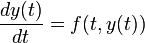
\includegraphics[scale=.6]{graphics/42ca594a14ebfe0d38675336c405ca1d.png}
% \caption{\textbackslash{}frac\{dy(t)\}\{dt\} = f(t,y(t))}
\end{figure}

with an initial value

\emph{y}(\emph{t}\textsubscript{0}) = \emph{y}\textsubscript{0}

To get a numeric solution, we replace the derivative on the LHS with a
finite difference approximation:

\begin{figure}[H]
\centering
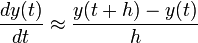
\includegraphics[scale=.6]{graphics/74ad42ba372e0541d6f14058e2c33c0f.png}
% \caption{\textbackslash{}frac\{dy(t)\}\{dt\} \textbackslash{}approx
% \textbackslash{}frac\{y(t+h)-y(t)\}\{h\}}
\end{figure}

then solve for \emph{y}(\emph{t} + \emph{h}):

\begin{figure}[H]
\centering
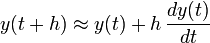
\includegraphics[scale=.6]{graphics/6ecb4a72d18052ff65e393b54c3850a2.png}
% \caption{y(t+h) \textbackslash{}approx y(t) + h \textbackslash{},
% \textbackslash{}frac\{dy(t)\}\{dt\}}
\end{figure}

which is the same as

\begin{figure}[H]
\centering
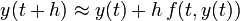
\includegraphics[scale=.6]{graphics/0a1294f5ac71c931e686c647d900fbcb.png}
% \caption{y(t+h) \textbackslash{}approx y(t) + h \textbackslash{},
% f(t,y(t))}
\end{figure}

The iterative solution rule is then:

\begin{figure}[H]
\centering
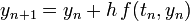
\includegraphics[scale=.6]{graphics/981cbbc69bfa735ea07313f59feba714.png}
% \caption{y\_\{n+1\} = y\_n + h \textbackslash{}, f(t\_n, y\_n)}
\end{figure}

\emph{h} is the step size, the most relevant parameter for accuracy of
the solution. A smaller step size increases accuracy but also the
computation cost, so it has always has to be hand-picked according to
the problem at hand.

\textbf{Example: Newton's Cooling Law}

Newton's cooling law describes how an object of initial temperature
\emph{T}(\emph{t}\textsubscript{0}) = \emph{T}\textsubscript{0} cools
down in an environment of temperature \emph{T}\textsubscript{\emph{R}}:

\begin{figure}[H]
\centering
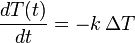
\includegraphics[scale=.6]{graphics/fca99b79cfa1b2d3a65395932e824f05.png}
% \caption{\textbackslash{}frac\{dT(t)\}\{dt\} = -k \textbackslash{},
% \textbackslash{}Delta T}
\end{figure}

or

\begin{figure}[H]
\centering
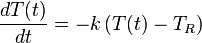
\includegraphics[scale=.6]{graphics/5028ac33d1b22df1c9509179c615ce6a.png}
% \caption{\textbackslash{}frac\{dT(t)\}\{dt\} = -k \textbackslash{},
% (T(t) - T\_R)}
\end{figure}

It says that the cooling rate
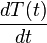
\includegraphics[scale=.6]{graphics/54f43bb3bb190844c7989f5864df1b2a.png}
of the object is proportional to the current temperature difference
Δ\emph{T} = (\emph{T}(\emph{t}) − \emph{T}\textsubscript{\emph{R}}) to
the surrounding environment.

The analytical solution, which we will compare to the numerical
approximation, is

\begin{figure}[H]
\centering
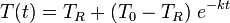
\includegraphics[scale=.6]{graphics/35fc97d739522cf3dc29d28cabc2e717.png}
% \caption{T(t) = T\_R + (T\_0 - T\_R) \textbackslash{}; e\^{}\{-k t\}}
\end{figure}

\textbf{Task}

The task is to implement a routine of Euler's method and then to use it
to solve the given example of Newton's cooling law with it for three
different step sizes of 2 s, 5 s and 10 s and to compare with the
analytical solution. The initial temperature \emph{T}\textsubscript{0}
shall be 100 °C, the room temperature \emph{T}\textsubscript{\emph{R}}
20 °C, and the cooling constant \emph{k} 0.07. The time interval to
calculate shall be from 0 s to 100 s.

A reference solution (\emph{Common Lisp}) can be seen on below. We see
that bigger step sizes lead to reduced approximation accuracy.

\begin{figure}[H]
\centering
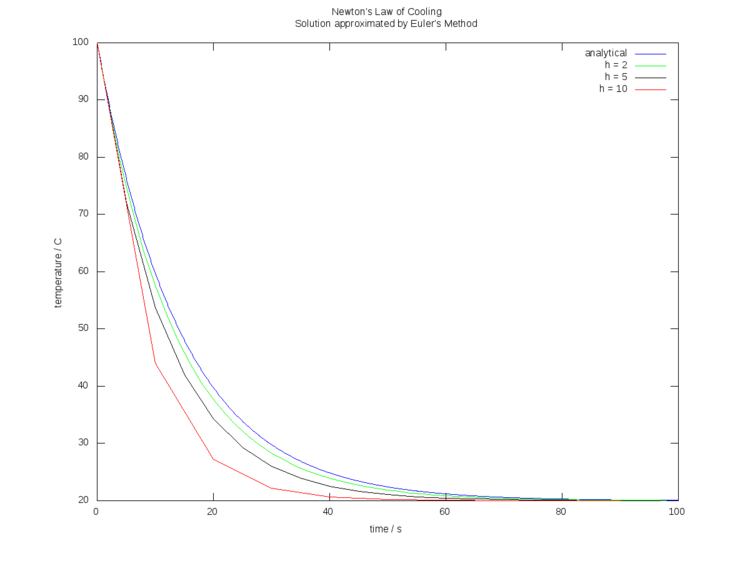
\includegraphics[scale=.6]{graphics/750px-Euler_Method_Newton_Cooling.png}
\end{figure}


\begin{wideverbatim}

(load "@lib/math.l")

(de euler (F Y A B H)
   (while (> B A)
      (prinl (round A) " " (round Y))
      (inc 'Y (*/ H (F A Y) 1.0))
      (inc 'A H) ) )

(de newtonCoolingLaw (A B)
   (*/ -0.07 (- B 20.) 1.0) )

(euler newtonCoolingLaw 100.0 0 100.0 2.0)
(euler newtonCoolingLaw 100.0 0 100.0 5.0)
(euler newtonCoolingLaw 100.0 0 100.0 10.0)

Output:

...
0.000 100.000
10.000 44.000
20.000 27.200
30.000 22.160
40.000 20.648
50.000 20.194
60.000 20.058
70.000 20.018
80.000 20.005
90.000 20.002

\end{wideverbatim}

\pagebreak{}
\section*{Evaluate binomial coefficients}

This programming task, is to calculate ANY binomial coefficient.

However, it has to be able to output

\includegraphics[scale=.6]{graphics/33a9aa45fa4dad1deffa8c921462ad74.png},
which is 10.

This formula is recommended:

\begin{figure}[H]
\centering
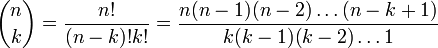
\includegraphics[scale=.6]{graphics/b7521c74cd98e492ade8dd3e9f40669a.png}
% \caption{\textbackslash{}binom\{n\}\{k\} =
% \textbackslash{}frac\{n!\}\{(n-k)!k!\} =
% \textbackslash{}frac\{n(n-1)(n-2)\textbackslash{}ldots(n-k+1)\}\{k(k-1)(k-2)\textbackslash{}ldots
% 1\}}
\end{figure}

\begin{wideverbatim}

(de binomial (N K)
   (let f '((N) (apply * (range 1 N)))
      (/ (f N) (* (f (- N K)) (f K))) ) )

Output:

: (binomial 5 3)
-> 10

\end{wideverbatim}

\pagebreak{}
\section*{Even or odd}

Test whether an integer is even or odd.

There is more than one way to solve this task:

\begin{itemize}
\item
  Use the even and odd predicates, if the language provides them.
\item Check the least significant digit. With binary integers, \emph{i
    \emph{bitwise-and} 1} equals 0
  \href{http://en.wiktionary.org/wiki/iff}{iff} \emph{i} is even, or
  equals 1 iff \emph{i} is odd.
\item
  Divide \emph{i} by 2. The remainder equals 0 iff \emph{i} is even. The
  remainder equals +1 or -1 iff \emph{i} is odd.
\item
  Use modular congruences:

  \begin{itemize}
  \item
    \emph{i} ≡ 0 (mod 2) iff \emph{i} is even.
  \item
    \emph{i} ≡ 1 (mod 2) iff \emph{i} is odd.
  \end{itemize}
\end{itemize}


\begin{wideverbatim}

  PicoLisp doesn't have a built-in predicate for that. Using
  '[http://software-lab.de/doc/refB.html#bit? bit?]' is the easiest
  and most efficient. The bit test with 1 will return NIL if the
  number is even.

: (bit? 1 3)
-> 1  # Odd

: (bit? 1 4)
-> NIL  # Even

\end{wideverbatim}

\pagebreak{}
\section*{Events}

\textbf{Event} is a synchronization object. An event has two states
\emph{signaled} and \emph{reset}. A \emph{task} may await for the
event to enter the desired state, usually the \emph{signaled} state.
It is released once the state is entered. Releasing waiting tasks is
called \emph{event notification}. Programmatically controlled events
can be set by a \emph{task} into one of its states.

In \emph{concurrent programming} event also refers to a notification
that some state has been reached through an asynchronous activity. The
source of the event can be:

\begin{itemize}
\item
  \emph{internal}, from another \emph{task},
  programmatically;
\item
  \emph{external}, from the hardware, such as user input, timer, etc.
  Signaling an event from the hardware is accomplished by means of
  hardware \emph{interrupts}.
\end{itemize}

Event is a low-level synchronization mechanism. It neither identify the
state that caused it signaled, nor the source of, nor who is the subject
of notification. Events augmented by data and/or publisher-subscriber
schemes are often referred as \textbf{messages}, \textbf{signals} etc.

In the context of general programming \textbf{event-driven
  architecture} refers to a design that deploy events in order to
synchronize \emph{tasks} with the asynchronous activities they must be
aware of. The opposite approach is \textbf{polling} sometimes called
\textbf{busy waiting}, when the synchronization is achieved by an
explicit periodic querying the state of the activity. As the name
suggests busy waiting consumes system resources even when the external
activity does not change its state.

Event-driven architectures are widely used in GUI design and SCADA
systems. They are flexible and have relatively short response times.
At the same time event-driven architectures suffer to the problems
related to their unpredictability. They face \emph{race condition},
deadlocking, live locks and priority inversion. For this reason
\emph{real-time} systems tend to polling schemes, trading performance
for predictability in the worst case scenario.

\begin{wideverbatim}

PicoLisp supports events from timers (via
'[http://software-lab.de/doc/refT.html#task task]' and
'[http://software-lab.de/doc/refA.html#alarm alarm]'),
file descriptors (also 'task') and various
'[http://software-lab.de/doc/refS.html#*Sig1 signals]'.
This will print a message after one second, then terminate the program after
another four seconds:

(alarm 1
   (prinl "Exit in 4 seconds")
   (alarm 4 (bye)) )

\end{wideverbatim}

\pagebreak{}
\section*{Evolutionary algorithm}

Starting with:

\begin{itemize}
\item
  The \texttt{target} string: \texttt{"METHINKS IT IS LIKE A WEASEL"}.
\item
  An array of random characters chosen from the set of upper-case
  letters together with the space, and of the same length as the target
  string. (Call it the \texttt{parent}).
\item
  A \texttt{fitness} function that computes the `closeness' of its
  argument to the target string.
\item
  A \texttt{mutate} function that given a string and a mutation rate
  returns a copy of the string, with some characters probably mutated.
\item
  While the \texttt{parent} is not yet the \texttt{target}:
\end{itemize}

\begin{itemize}
\item
  copy the \texttt{parent} C times, each time allowing some random
  probability that another character might be substituted using
  \texttt{mutate}.
\item
  Assess the \texttt{fitness} of the parent and all the copies to the
  \texttt{target} and make the most fit string the new \texttt{parent},
  discarding the others.
\item
  repeat until the parent converges, (hopefully), to the target.
\end{itemize}

Cf:
\href{http://en.wikipedia.org/wiki/Weasel\_program\#Weasel\_algorithm}{Weasel
algorithm} and
\href{http://en.wikipedia.org/wiki/Evolutionary\_algorithm}{Evolutionary
algorithm}

Note: to aid comparison, try and ensure the variables and functions
mentioned in the task description appear in solutions


\begin{wideverbatim}
This example uses 'gen', the genetic function in "lib/simul.l"

(load "@lib/simul.l")

(setq *Target (chop "METHINKS IT IS LIKE A WEASEL"))

# Generate random character
(de randChar ()
   (if (=0 (rand 0 26))
      " "
      (char (rand `(char "A") `(char "Z"))) ) )

# Fitness function (Hamming distance)
(de fitness (A)
   (cnt = A *Target) )

# Genetic algorithm
(gen
   (make                               # Parent population
      (do 100                             # C = 100 children
         (link
            (make
               (do (length *Target)
                  (link (randChar)) ) ) ) ) )
   '((A)                               # Termination condition
      (prinl (maxi fitness A))            # Print the fittest element
      (member *Target A) )                # and check if solution is found
   '((A B)                             # Recombination function
      (mapcar
         '((C D) (if (rand T) C D))       # Pick one of the chars
         A B ) )
   '((A)                               # Mutation function
      (mapcar
         '((C)
            (if (=0 (rand 0 10))          # With a proability of 10\%
               (randChar)                 # generate a new char, otherwise
               C ) )                      # return the current char
         A ) )
   fitness )                           # Selection function

Output:

RQ ASLWWWI ANSHPNABBAJ ZLTKX
DETGGNGHWITIKSXLIIEBA WAATPC
CETHINWS ITKESQGIKE A WSAGHO
METHBNWS IT NSQLIKE A WEAEWL
METHINKS IT ISCLIKE A WVASEL
METHINKS IT ISOLIKE A WEASEL
METHINKS IT IS LIKE A WEASEL

\end{wideverbatim}

\pagebreak{}
\section*{Exceptions}

\textbf{Control Structures}

These are examples of \emph{control structures}. You may also be
interested in:

\begin{itemize}
\item
  \emph{Conditional structures}
\item
  \textbf{Exceptions}
\item
  \emph{Flow-control structures}
\item
  \emph{Loops}
\end{itemize}

This task is to give an example of an exception handling routine and to
``throw'' a new exception.

Cf. \emph{Exceptions Through Nested Calls}


\begin{wideverbatim}

  [http://software-lab.de/doc/refC.html#catch catch],
  [http://software-lab.de/doc/refT.html#throw throw] (and
  [http://software-lab.de/doc/refF.html#finally finally]) can be used
  for exception handling. 'throw' will transfer control to a 'catch'
  environment that was set up with the given label.

(catch 'thisLabel          # Catch this label
   (println 1)             # Do some processing (print '1')
   (throw 'thisLabel 2)    # Abort processing and return '2'
   (println 3) )           # This is never reached

Output:

1        # '1' is printed
-> 2     # '2' is returned

\end{wideverbatim}

\pagebreak{}
\section*{Exceptions/Catch an exception thrown in a nested call}

Show how to create a user-defined exception and show how to catch an
exception raised from several nested calls away.

\begin{enumerate}
\item
  Create two user-defined exceptions, U0 and U1.
\item
  Have function foo call function bar twice.
\item
  Have function bar call function baz.
\item
  Arrange for function baz to raise, or throw exception U0 on its first
  call, then exception U1 on its second.
\item
  Function foo should catch only exception U0, not U1.
\end{enumerate}

Show/describe what happens when the program is run.


\begin{wideverbatim}

(de foo ()
   (for Tag '(U0 U1)
      (catch 'U0
         (bar Tag) ) ) )

(de bar (Tag)
   (baz Tag) )

(de baz (Tag)
   (throw Tag) )

(mapc trace '(foo bar baz))
(foo)

Output:

 foo :
  bar : U0
   baz : U0
  bar : U1
   baz : U1
[x:13] !? (throw Tag)
U1 -- Tag not found
?                          # Debug prompt

\end{wideverbatim}

\pagebreak{}
\section*{Executable library}

The general idea behind an executable library is to create a library
that when used as a library does one thing; but has the ability to be
run directly via command line. Thus the API comes with a CLI in the very
same source code file.

\textbf{Task detail}

\begin{itemize}
\item Create a library/module/dll/shared object/\ldots{} for a
  programming language that contains a function/method called
  hailstone that is a function taking a positive integer and returns
  the \emph{Hailstone sequence} for that number.
\end{itemize}

\begin{itemize}
\item The library, when executed directly should satisfy the remaining
  requirements of the \emph{Hailstone sequence} task:
\end{itemize}

2. Use the routine to show that the hailstone sequence for the number
27 has 112 elements starting with 27, 82, 41, 124 and ending with 8,
4, 2, 1

3. Show the number less than 100,000 which has the longest hailstone
sequence together with that sequences length.

\begin{itemize}
\item
  Create a second executable to calculate the following:

  \begin{itemize}
  \item
    Use the libraries hailstone function, in the standard manner, (or
    document how this use deviates from standard use of a library),
    together with extra code in this executable, to find the hailstone
    length returned most often for 1 \textless{}= n \textless{} 100,000"
  \end{itemize}
\end{itemize}

\begin{itemize}
\item
  Explain any extra setup/run steps needed to complete the task.
\end{itemize}

\textbf{Notes:}

\begin{itemize}
\item
  It is assumed that for a language that overwhelmingly ships in a
  compiled form, such as C, the library must also be an executable and
  the compiled user of that library is to do so without changing the
  compiled library. I.e. the compile tool-chain is assumed \emph{not} to
  be present in the runtime environment.
\item
  Interpreters are present in the runtime environment.
\end{itemize}


\begin{wideverbatim}

There is no formal difference between libraries and other executable files in
PicoLisp. Any function in a library can be called from the command line by
prefixing it with '-'. Create an executable file (chmod +x) "hailstone.l":

#!/usr/bin/picolisp /usr/lib/picolisp/lib.l

(de hailstone (N)
   (make
      (until (= 1 (link N))
         (setq N
            (if (bit? 1 N)
               (inc (* N 3))
               (/ N 2) ) ) ) ) )

(de hailtest ()
   (let L (hailstone 27)
      (test 112 (length L))
      (test (27 82 41 124) (head 4 L))
      (test (8 4 2 1) (tail 4 L)) )
   (let N (maxi '((N) (length (hailstone N))) (range 1 100000))
      (test 77031 N)
      (test 351 (length (hailstone N))) )
   (println 'OK)
   (bye) )

and an executable file (chmod +x) "test.l":

#!/usr/bin/picolisp /usr/lib/picolisp/lib.l

(load "hailstone.l")

(let Len NIL
   (for N 100000
      (accu 'Len (length (hailstone N)) 1) )
   (let M (maxi cdr Len)
      (prinl "The hailstone length returned most often is " (car M))
      (prinl "It is returned " (cdr M) " times") ) )
(bye)

Test:

\$ ./hailstone.l -hailtest
OK

\$ ./test.l
The hailstone length returned most often is 72
It is returned 1467 times

\end{wideverbatim}

\pagebreak{}
\section*{Execute Brain****}

\textbf{Execute Brain****} is an \textbf{implementation} of
\emph{Brainf***}. 

An implementation need only properly implement the `{[}', '{]}', `+',
'-', `\textless{}', `\textgreater{}', ',', and '.' instructions. Any
cell size is allowed, EOF support is optional, as is whether you have
bounded or unbounded memory.


\begin{wideverbatim}

This solution uses a doubly-linked list for the cell space. That list consists
of a single cell initially, and grows automatically in both directions. The
value in each cell is unlimited.

(off "Program")

(de compile (File)
   (let Stack NIL
      (setq "Program"
         (make
            (in File
               (while (char)
                  (case @
                     (">"
                        (link
                           '(setq Data
                              (or
                                 (cddr Data)
                                 (con (cdr Data) (cons 0 (cons Data))) ) ) ) )
                     ("<"
                        (link
                           '(setq Data
                              (or
                                 (cadr Data)
                                 (set (cdr Data) (cons 0 (cons NIL Data))) ) ) ) )
                     ("+" (link '(inc Data)))
                     ("-" (link '(dec Data)))
                     ("." (link '(prin (char (car Data)))))
                     ("," (link '(set Data (char (read)))))
                     ("["
                        (link
                           '(setq Code
                              ((if (=0 (car Data)) cdar cdr) Code) ) )
                        (push 'Stack (chain (cons))) )
                     ("]"
                        (unless Stack
                           (quit "Unbalanced ']'") )
                        (link
                           '(setq Code
                              ((if (n0 (car Data)) cdar cdr) Code) ) )
                        (let (There (pop 'Stack)  Here (cons There))
                           (chain (set There Here)) ) ) ) ) ) ) )
      (when Stack
         (quit "Unbalanced '['") ) ) )

(de execute ()
   (let Data (cons 0 (cons))              # Create initial cell
      (for (Code "Program"  Code)         # Run program
         (eval (pop 'Code)) )
      (while (cadr Data)                  # Find beginning of data
         (setq Data @) )
      (filter prog Data '(T NIL .)) ) )   # Return data space

\end{wideverbatim}

\begin{wideverbatim}


Output:

: (compile "hello.bf")
-> NIL

: (execute)
Goodbye, World!
-> (0 10 33 44 71 87 98 100 114 121)

\end{wideverbatim}

\pagebreak{}
\section*{Execute HQ9+}

Implement a \emph{HQ9+} interpreter or compiler for Rosetta Code.


\begin{wideverbatim}

(de hq9+ (Code)
   (let Accu 0
      (for C (chop Code)
         (case C
            ("H" (prinl "Hello, world"))
            ("Q" (prinl Code))
            ("9"
               (for (N 99 (gt0 N))
                  (prinl N " bottles of beer on the wall")
                  (prinl N " bottles of beer")
                  (prinl "Take one down, pass it around")
                  (prinl (dec 'N) " bottles of beer on the wall")
                  (prinl) ) )
            ("+" (inc 'Accu)) ) )
      Accu ) )

\end{wideverbatim}

\pagebreak{}
\section*{Execute a Markov algorithm}

Create an interpreter for a
\href{http://en.wikipedia.org/wiki/Markov\_algorithm}{Markov
  Algorithm}. Rules have the syntax:

\begin{wideverbatim}
<ruleset> ::= ((<comment> | <rule>) <newline>+)*
<comment> ::= # {<any character>}
<rule> ::= <pattern> <whitespace> -> <whitespace> [.] <replacement>
<whitespace> ::= (<tab> | <space>) [<whitespace>]
\end{wideverbatim}

There is one rule per line. If there is a . present before the
\textless{}replacement\textgreater{}, then this is a terminating rule
in which case the interpreter must halt execution. A ruleset consists
of a sequence of rules, with optional comments.


\begin{wideverbatim}

(de markov (File Text)
   (use (@A @Z R)
      (let Rules
         (make
            (in File
               (while (skip "#")
                  (when (match '(@A " " "-" ">" " " @Z) (replace (line) "@" "#"))
                     (link (cons (clip @A) (clip @Z))) ) ) ) )
         (setq Text (chop Text))
         (pack
            (loop
               (NIL
                  (find
                     '((R) (match (append '(@A) (car R) '(@Z)) Text))
                     Rules )
                  Text )
               (T (= "." (cadr (setq R @)))
                  (append @A (cddr R) @Z) )
               (setq Text (append @A (cdr R) @Z)) ) ) ) ) )

Output:

: (markov "r1" "I bought a B of As from T S.")
-> "I bought a bag of apples from my brother."

: (markov "r2" "I bought a B of As from T S.")
-> "I bought a bag of apples from T shop."

: (markov "r3" "I bought a B of As W my Bgage from T S.")
-> "I bought a bag of apples with my money from T shop."

: (markov "r4" "_1111*11111_")
-> "11111111111111111111"

: (markov "r5" "000000A000000")
-> "00011H1111000"

\end{wideverbatim}

\pagebreak{}
\section*{Execute a system command}

In this task, the goal is to run either the \texttt{ls} (\texttt{dir} on
Windows) system command, or the \texttt{pause} system command.

\begin{wideverbatim}

(call "ls")

\end{wideverbatim}

\pagebreak{}
\section*{Exponentiation operator}

Most all programming languages have a built-in implementation of
exponentiation. Re-implement integer exponentiation for both
int\textsuperscript{int} and float\textsuperscript{int} as both a
procedure, and an operator (if your language supports operator
definition).

If the language supports operator (or procedure) overloading, then an
overloaded form should be provided for both int\textsuperscript{int} and
float\textsuperscript{int} variants.


\begin{wideverbatim}

  This uses Knuth's algorithm (The Art of Computer Programming, Vol.
  2, page 442)

(de ** (X N)  # N th power of X
   (let Y 1
      (loop
         (when (bit? 1 N)
            (setq Y (* Y X)) )
         (T (=0 (setq N (>> 1 N)))
            Y )
         (setq X (* X X)) ) ) )

\end{wideverbatim}

\pagebreak{}
\section*{Extend your language}

\textbf{Control Structures}

These are examples of \emph{control structures}. You may also be
interested in:

\begin{itemize}
\item
 \emph{Conditional structures}
\item
  \emph{Exceptions}
\item
  \emph{Flow-control structures}
\item
  \emph{Loops}
\end{itemize}

Some programming languages allow you to
\href{http://en.wikipedia.org/wiki/Extensible\_programming}{extend}
the language. While this can be done to a certain degree in most
languages (e.g. by using macros), other languages go much further.
Most notably in the Forth and Lisp families, programming per se is
done by extending the language without any formal distinction between
built-in and user-defined elements.

If your language supports it, show how to introduce a new flow control
mechanism. A practical and useful example is a four-way branch:

Occasionally, code must be written that depends on \emph{two}
conditions, resulting in up to four branches (depending on whether both,
only the first, only the second, or none of the conditions are
``true''). In a C-like language this could look like the following:

\begin{verbatim}
  if (condition1isTrue) {
     if (condition2isTrue)
        bothConditionsAreTrue();
     else
        firstConditionIsTrue();
  }
  else if (condition2isTrue)
     secondConditionIsTrue();
  else
     noConditionIsTrue();
\end{verbatim}

Besides being rather cluttered, the statement(s) for `condition2isTrue'
must be written down twice. If `condition2isTrue' were a lengthy and
involved expression, it would be quite unreadable, and the code
generated by the compiler might be unnecessarily large.

This can be improved by introducing a new keyword \textbf{if2}. It is
similar to \textbf{if}, but takes two conditional statements instead of
one, and up to three `else' statements. One proposal (in pseudo-C
syntax) might be:

\begin{verbatim}
  if2 (condition1isTrue) (condition2isTrue)
     bothConditionsAreTrue();
  else1
     firstConditionIsTrue();
  else2
     secondConditionIsTrue();
  else
     noConditionIsTrue();
\end{verbatim}

Pick the syntax which suits your language. The keywords `else1' and
`else2' are just examples. The new conditional expression should look,
nest and behave analog to the language's built-in `if' statement.


\begin{wideverbatim}

(undef 'if2)  # Undefine the built-in 'if2'

(de if2 "P"
   (if (eval (pop '"P"))
      (eval ((if (eval (car "P")) cadr caddr) "P"))
      (if (eval (car "P"))
         (eval (cadddr "P"))
         (run (cddddr "P")) ) ) )

Usage:

(if2 (condition1isTrue) (condition2isTrue)
   (bothConditionsAreTrue)             # A single expression in each of the
   (firstConditionIsTrue)              # first three branches
   (secondConditionIsTrue)
   (noConditionIsTrue)                 # The final branch may contain
   (...) )                             # an arbitrary number of expressions

As another example of language extension, see [[Anonymous recursion#PicoLisp]].

\end{wideverbatim}

\pagebreak{}
\section*{Extreme floating point values}

The IEEE floating point specification defines certain `extreme' floating
point values such as minus zero, -0.0, a value distinct from plus zero;
not a number, NaN; and plus and minus infinity.

The task is to use expressions involving other `normal' floating point
values in your language to calculate these, (and maybe other), extreme
floating point values in your language and assign them to variables.
Print the values of these variables if possible; and show some
arithmetic with these values and variables. If your language can
directly enter these extreme floating point values then show it.

C.f:

\begin{itemize}
\item
  \href{http://www-users.math.umd.edu/~jkolesar/mait613/floating\_point\_math.pdf}{What
  Every Computer Scientist Should Know About Floating-Point Arithmetic}
\item
  \emph{Infinity}
\item
  \emph{Detect division by zero}
\item
  \emph{Literals/Floating point}
\end{itemize}


\begin{wideverbatim}

  PicoLisp has only very limited built-in floating point support, and
  handles the rest by calling native (typically C) libraries. Minus
  zero and negative infinity cannot be represented, while NaN is
  represented by NIL

(load "@lib/math.l")

: (exp 1000.0)  # Too large for IEEE floats
-> T

: (+ 1 2 NIL 3)  # NaN propagates
-> NIL

\end{wideverbatim}



% %%%%%%%%%%%%%%%%%%%%%%%% referenc.tex %%%%%%%%%%%%%%%%%%%%%%%%%%%%%%
% sample references
% %
% Use this file as a template for your own input.
%
%%%%%%%%%%%%%%%%%%%%%%%% Springer-Verlag %%%%%%%%%%%%%%%%%%%%%%%%%%
%
% BibTeX users please use
% \bibliographystyle{}
% \bibliography{}
%
\biblstarthook{In view of the parallel print and (chapter-wise) online publication of your book at \url{www.springerlink.com} it has been decided that -- as a genreral rule --  references should be sorted chapter-wise and placed at the end of the individual chapters. However, upon agreement with your contact at Springer you may list your references in a single seperate chapter at the end of your book. Deactivate the class option \texttt{sectrefs} and the \texttt{thebibliography} environment will be put out as a chapter of its own.\\\indent
References may be \textit{cited} in the text either by number (preferred) or by author/year.\footnote{Make sure that all references from the list are cited in the text. Those not cited should be moved to a separate \textit{Further Reading} section or chapter.} The reference list should ideally be \textit{sorted} in alphabetical order -- even if reference numbers are used for the their citation in the text. If there are several works by the same author, the following order should be used: 
\begin{enumerate}
\item all works by the author alone, ordered chronologically by year of publication
\item all works by the author with a coauthor, ordered alphabetically by coauthor
\item all works by the author with several coauthors, ordered chronologically by year of publication.
\end{enumerate}
The \textit{styling} of references\footnote{Always use the standard abbreviation of a journal's name according to the ISSN \textit{List of Title Word Abbreviations}, see \url{http://www.issn.org/en/node/344}} depends on the subject of your book:
\begin{itemize}
\item The \textit{two} recommended styles for references in books on \textit{mathematical, physical, statistical and computer sciences} are depicted in ~\cite{science-contrib, science-online, science-mono, science-journal, science-DOI} and ~\cite{phys-online, phys-mono, phys-journal, phys-DOI, phys-contrib}.
\item Examples of the most commonly used reference style in books on \textit{Psychology, Social Sciences} are~\cite{psysoc-mono, psysoc-online,psysoc-journal, psysoc-contrib, psysoc-DOI}.
\item Examples for references in books on \textit{Humanities, Linguistics, Philosophy} are~\cite{humlinphil-journal, humlinphil-contrib, humlinphil-mono, humlinphil-online, humlinphil-DOI}.
\item Examples of the basic Springer style used in publications on a wide range of subjects such as \textit{Computer Science, Economics, Engineering, Geosciences, Life Sciences, Medicine, Biomedicine} are ~\cite{basic-contrib, basic-online, basic-journal, basic-DOI, basic-mono}. 
\end{itemize}
}

\begin{thebibliography}{99.}%
% and use \bibitem to create references.
%
% Use the following syntax and markup for your references if 
% the subject of your book is from the field 
% "Mathematics, Physics, Statistics, Computer Science"
%
% Contribution 
\bibitem{science-contrib} Broy, M.: Software engineering --- from auxiliary to key technologies. In: Broy, M., Dener, E. (eds.) Software Pioneers, pp. 10-13. Springer, Heidelberg (2002)
%
% Online Document
\bibitem{science-online} Dod, J.: Effective substances. In: The Dictionary of Substances and Their Effects. Royal Society of Chemistry (1999) Available via DIALOG. \\
\url{http://www.rsc.org/dose/title of subordinate document. Cited 15 Jan 1999}
%
% Monograph
\bibitem{science-mono} Geddes, K.O., Czapor, S.R., Labahn, G.: Algorithms for Computer Algebra. Kluwer, Boston (1992) 
%
% Journal article
\bibitem{science-journal} Hamburger, C.: Quasimonotonicity, regularity and duality for nonlinear systems of partial differential equations. Ann. Mat. Pura. Appl. \textbf{169}, 321--354 (1995)
%
% Journal article by DOI
\bibitem{science-DOI} Slifka, M.K., Whitton, J.L.: Clinical implications of dysregulated cytokine production. J. Mol. Med. (2000) doi: 10.1007/s001090000086 
%
\bigskip

% Use the following (APS) syntax and markup for your references if 
% the subject of your book is from the field 
% "Mathematics, Physics, Statistics, Computer Science"
%
% Online Document
\bibitem{phys-online} J. Dod, in \textit{The Dictionary of Substances and Their Effects}, Royal Society of Chemistry. (Available via DIALOG, 1999), 
\url{http://www.rsc.org/dose/title of subordinate document. Cited 15 Jan 1999}
%
% Monograph
\bibitem{phys-mono} H. Ibach, H. L\"uth, \textit{Solid-State Physics}, 2nd edn. (Springer, New York, 1996), pp. 45-56 
%
% Journal article
\bibitem{phys-journal} S. Preuss, A. Demchuk Jr., M. Stuke, Appl. Phys. A \textbf{61}
%
% Journal article by DOI
\bibitem{phys-DOI} M.K. Slifka, J.L. Whitton, J. Mol. Med., doi: 10.1007/s001090000086
%
% Contribution 
\bibitem{phys-contrib} S.E. Smith, in \textit{Neuromuscular Junction}, ed. by E. Zaimis. Handbook of Experimental Pharmacology, vol 42 (Springer, Heidelberg, 1976), p. 593
%
\bigskip
%
% Use the following syntax and markup for your references if 
% the subject of your book is from the field 
% "Psychology, Social Sciences"
%
%
% Monograph
\bibitem{psysoc-mono} Calfee, R.~C., \& Valencia, R.~R. (1991). \textit{APA guide to preparing manuscripts for journal publication.} Washington, DC: American Psychological Association.
%
% Online Document
\bibitem{psysoc-online} Dod, J. (1999). Effective substances. In: The dictionary of substances and their effects. Royal Society of Chemistry. Available via DIALOG. \\
\url{http://www.rsc.org/dose/Effective substances.} Cited 15 Jan 1999.
%
% Journal article
\bibitem{psysoc-journal} Harris, M., Karper, E., Stacks, G., Hoffman, D., DeNiro, R., Cruz, P., et al. (2001). Writing labs and the Hollywood connection. \textit{J Film} Writing, 44(3), 213--245.
%
% Contribution 
\bibitem{psysoc-contrib} O'Neil, J.~M., \& Egan, J. (1992). Men's and women's gender role journeys: Metaphor for healing, transition, and transformation. In B.~R. Wainrig (Ed.), \textit{Gender issues across the life cycle} (pp. 107--123). New York: Springer.
%
% Journal article by DOI
\bibitem{psysoc-DOI}Kreger, M., Brindis, C.D., Manuel, D.M., Sassoubre, L. (2007). Lessons learned in systems change initiatives: benchmarks and indicators. \textit{American Journal of Community Psychology}, doi: 10.1007/s10464-007-9108-14.
%
%
% Use the following syntax and markup for your references if 
% the subject of your book is from the field 
% "Humanities, Linguistics, Philosophy"
%
\bigskip
%
% Journal article
\bibitem{humlinphil-journal} Alber John, Daniel C. O'Connell, and Sabine Kowal. 2002. Personal perspective in TV interviews. \textit{Pragmatics} 12:257--271
%
% Contribution 
\bibitem{humlinphil-contrib} Cameron, Deborah. 1997. Theoretical debates in feminist linguistics: Questions of sex and gender. In \textit{Gender and discourse}, ed. Ruth Wodak, 99--119. London: Sage Publications.
%
% Monograph
\bibitem{humlinphil-mono} Cameron, Deborah. 1985. \textit{Feminism and linguistic theory.} New York: St. Martin's Press.
%
% Online Document
\bibitem{humlinphil-online} Dod, Jake. 1999. Effective substances. In: The dictionary of substances and their effects. Royal Society of Chemistry. Available via DIALOG. \\
http://www.rsc.org/dose/title of subordinate document. Cited 15 Jan 1999
%
% Journal article by DOI
\bibitem{humlinphil-DOI} Suleiman, Camelia, Daniel C. O�Connell, and Sabine Kowal. 2002. `If you and I, if we, in this later day, lose that sacred fire...�': Perspective in political interviews. \textit{Journal of Psycholinguistic Research}. doi: 10.1023/A:1015592129296.
%
%
%
\bigskip
%
%
% Use the following syntax and markup for your references if 
% the subject of your book is from the field 
% "Computer Science, Economics, Engineering, Geosciences, Life Sciences"
%
%
% Contribution 
\bibitem{basic-contrib} Brown B, Aaron M (2001) The politics of nature. In: Smith J (ed) The rise of modern genomics, 3rd edn. Wiley, New York 
%
% Online Document
\bibitem{basic-online} Dod J (1999) Effective Substances. In: The dictionary of substances and their effects. Royal Society of Chemistry. Available via DIALOG. \\
\url{http://www.rsc.org/dose/title of subordinate document. Cited 15 Jan 1999}
%
% Journal article by DOI
\bibitem{basic-DOI} Slifka MK, Whitton JL (2000) Clinical implications of dysregulated cytokine production. J Mol Med, doi: 10.1007/s001090000086
%
% Journal article
\bibitem{basic-journal} Smith J, Jones M Jr, Houghton L et al (1999) Future of health insurance. N Engl J Med 965:325--329
%
% Monograph
\bibitem{basic-mono} South J, Blass B (2001) The future of modern genomics. Blackwell, London 
%
\end{thebibliography}

